\documentclass{beamer}
\usepackage{xeCJK}
\usetheme{Berlin}
\usecolortheme{seahorse}

\title{后缀自动机(SAM)}
\author{fjy666}
\date{June 16th, 2022}

\begin{document}
    \frame{\titlepage}

    \section{Introduce}
    \begin{frame}
        \frametitle{引入}
        首先,SAM 是什么? \\
        Suffix AutoMaton,后缀自动机。\\
        这是 OI 中字符串算法的最高点了。\\
        虽然如此,我们要清楚一个概念:\\
        \bf SAM 和 SA(后缀数组) 没有任何关系。\\  
        \textnormal{那么,就开始吧!}
    \end{frame}

    \begin{frame}
        \frametitle{介绍}
        SAM 是一种什么结构?\\  
        我们先不管它,先来看一个东西:\\
        字符串 S=\texttt{"bab"} 和它的「后缀 Trie」(即把所有后缀扔到一个 Trie 上)
        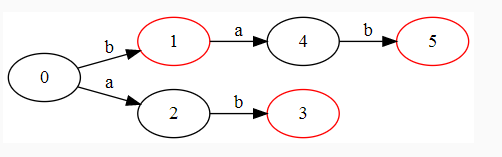
\includegraphics[height=3cm]{g1.png}
    \end{frame}

    \begin{frame}
        \frametitle{介绍}
        这玩意有个非常棒的性质:它包括了 S 的所有子串的信息。\\
        从节点 $0$ 开始,随便走一段必定是 S 的子串,\\
        而 S 的子串也必定是 $0$ 到某一个节点的路径。\\
        并且,这个「后缀 Trie」是一个 DAG,可以很方便的 dp。\\
        \pause
        唯一也是致命的缺点:这玩意的时空复杂度是 $\mathcal{O}(n^2)$ 的!\\
        看到这里,你应该清楚 SAM 是个什么东西了吧!
    \end{frame}

    \begin{frame}
        没错,SAM 就是一个具有上述性质,并且时空复杂度均为 $\mathcal{O}(n\log\Sigma)$ 的结构!
    \end{frame}

    \section*{概念}

    \begin{frame}
        \frametitle{定义}
        虽说如此,SAM 的概念还是有必要提一句的。  \\
        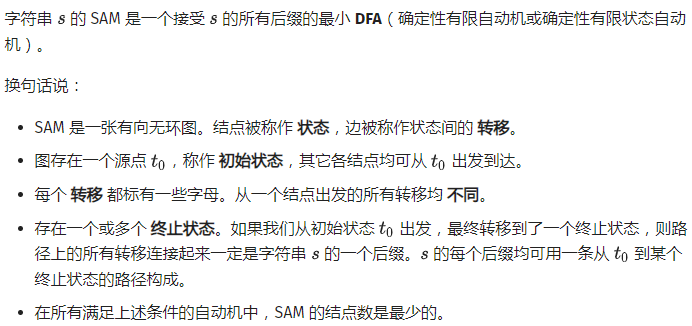
\includegraphics[height=5cm]{g2.png} \\
        From oi-wiki.org

    \end{frame}

    \begin{frame}
        \frametitle{endpos}
        endpos 是什么?\\
        考虑原串 S 的任意非空子串 T,那么\\
        endpos(T) 被定义为 T 在 S 中出现时末尾位置所组成的集合(下标从 1 开始)。\\
        这个可能有点难懂,所以我举个例子:\\
        S = \texttt{"114514"}\textnormal,T=\texttt"14",\\
        那么 endpos(T)=\{3,6\}。\\
        对于空串,我们定义它的 endpos 为 \{0,1,2,3,$\cdots$,|S|\}\\
        是不是非常 Easy?这玩意必须记住,这是重中之重。
    \end{frame}

    \begin{frame}
        \frametitle{node}
        自动机吗,肯定是有一个个节点组成的。\\
        那么 SAM 的节点是什么呢?\\

    \end{frame}

    \section*{Summary}

    \begin{frame}
        \frametitle{总结}
        SAM 确实是一种比较强大的 string DS。  \\
        它可以很方便地解决很多和后缀有关的东西。\\
        有些本质不同子串问题也可以用它。\\
        总而言之,遇到不会的题,SAM 淦它就对了!
    \end{frame}

    \begin{frame}
        \frametitle{Goodbye}
        Thank you for your listening!\\
        Made by fjy666.\\
        参考链接:\\
        https://oi-wiki.org/string/sam/ \\
        https://www.luogu.com.cn/problem/solution/P3804 \\
        https://alpha1022.gitee.io/sam-visualizer/ \\
        https://blog.csdn.net/qq\_42101694/article/details/111740597
    \end{frame}

    \begin{frame}
        \frametitle{Special Thanks}
        Special Thanks to lym(fix \LaTeX\ error in my computer), the oi-wiki and luogu.
    \end{frame}
\end{document}